\chapter{Adding Openstack Users}
In this section, we will add user accounts in Keystone that can
use Openstack System.
%Intro\footnotemark\\
\begin{spacing}{1.2}
%note en bas de page

\par So we will first create a project:
\\
\begin{figure}[!htb] 
\begin{center} 
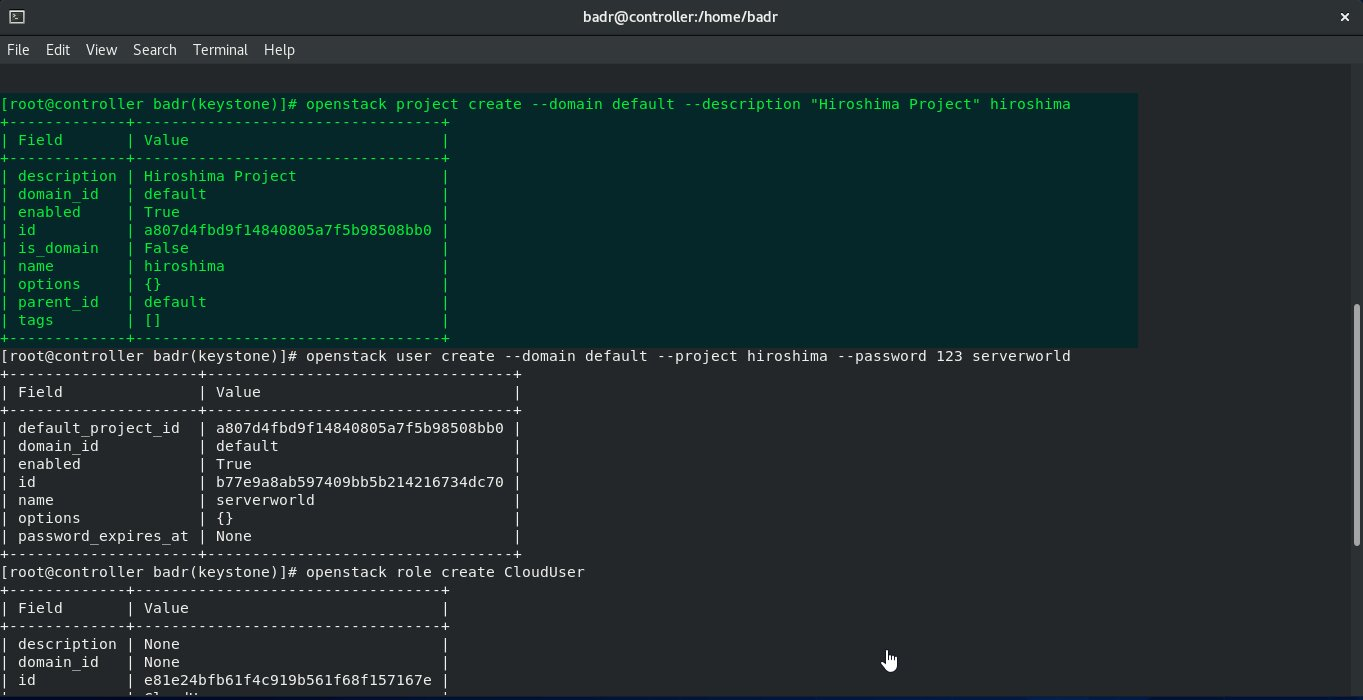
\includegraphics[width=1\linewidth]{Cloud/Adding Openstack Users/add a project} 
\end{center} 
\caption{add a project} 
\end{figure} 
\FloatBarrier
\\

\par Then we add a user named serverworld:
\\
\begin{figure}[!htb] 
\begin{center} 
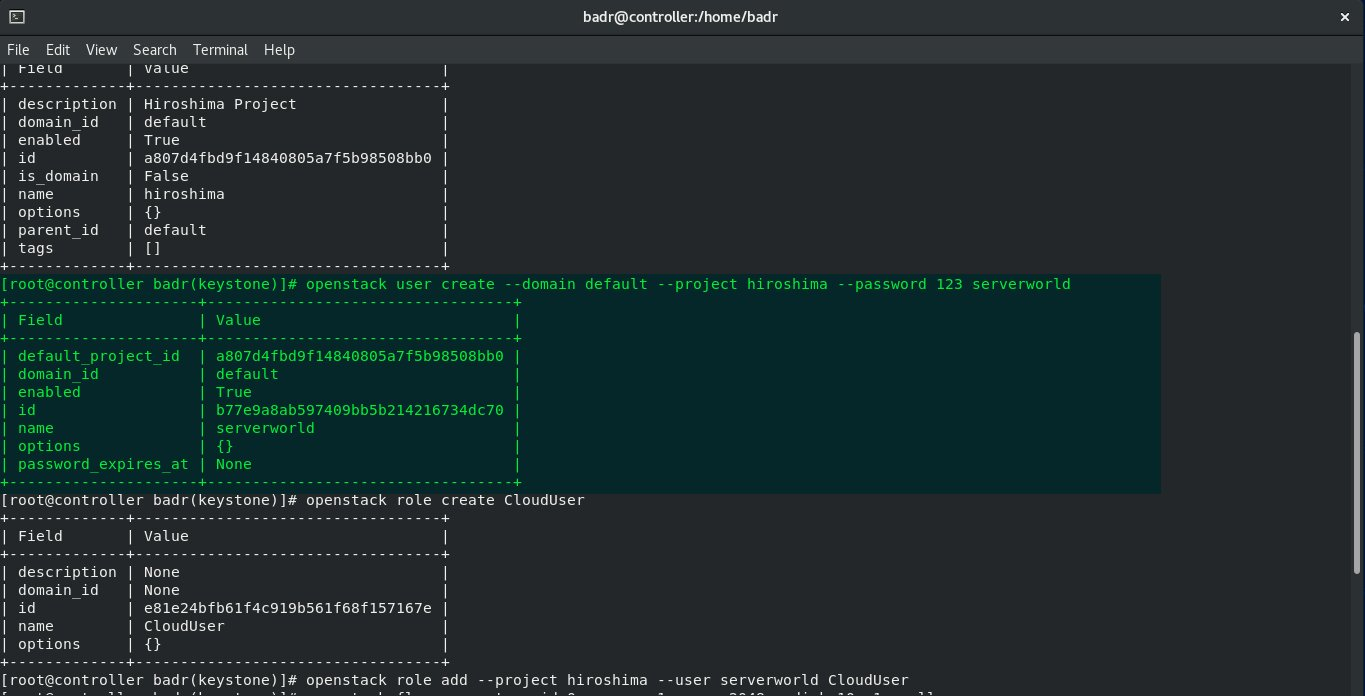
\includegraphics[width=1\linewidth]{Cloud/Adding Openstack Users/add a user} 
\end{center} 
\caption{add a user} 
\end{figure} 
\FloatBarrier


\par After that, we will create a role, so that we can add the created user to the role. And
we can add flavors which define the vCPU or the memory of an instance.
\\
\begin{figure}[!htb] 
\begin{center} 
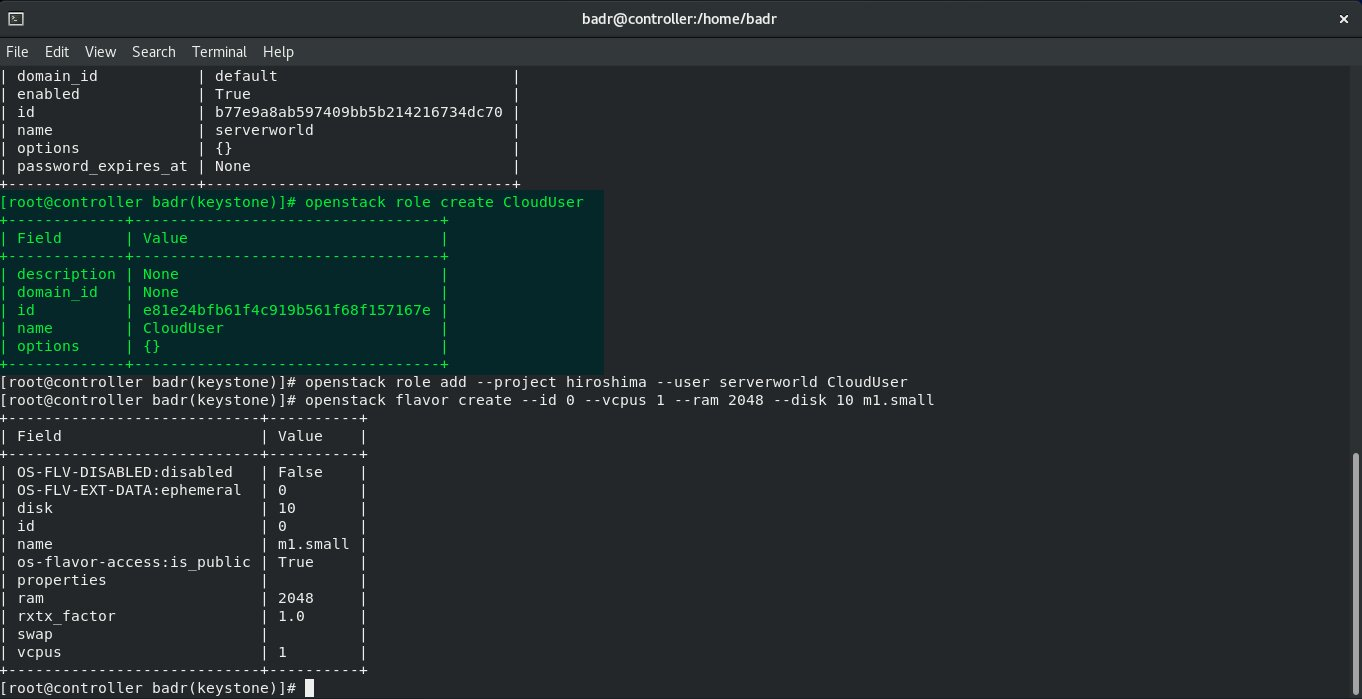
\includegraphics[width=1\linewidth]{Cloud/Adding Openstack Users/add a role} 
\end{center} 
\caption{add a role} 
\end{figure} 
\FloatBarrier
\\
\begin{figure}[!htb] 
\begin{center} 
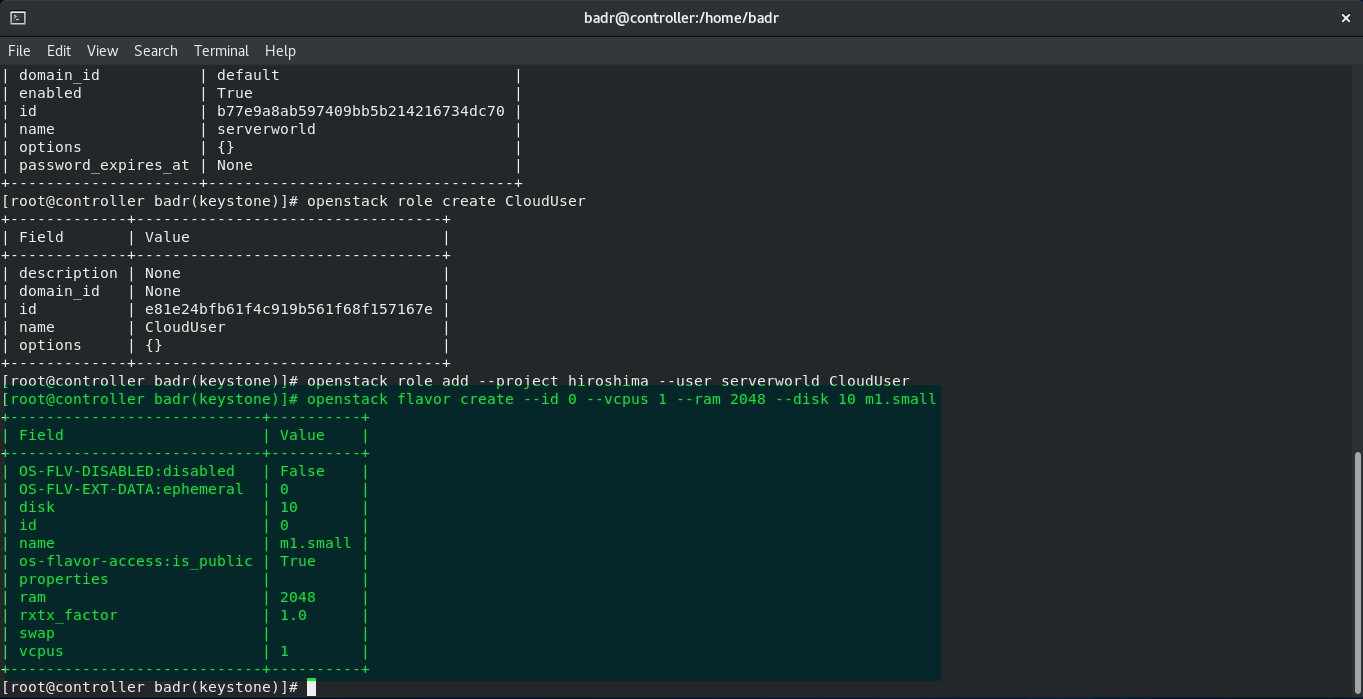
\includegraphics[width=1\linewidth]{Cloud/Adding Openstack Users/add [flavor]} 
\end{center} 
\caption{add [flavor]} 
\end{figure} 
\FloatBarrier
\\


\end{spacing}